% !TEX TS-program = XeLaTeX
% !TEX encoding = UTF-8 Unicode

\chapter{系统相关技术}
\label{chap04}
\defaultfont

\section{Spring Boot介绍}

Spring Boot可以更快创建独立的、基于Spring的生产级应用。该框架解决了Spring框架配置非常繁琐的问题,简化了项目开发流程\cite{.2019f}。

\begin{enumerate}
    \item 创建独立的Spring应用程序。
    \item 直接嵌入Tomcat、Jetty或Undertow(不需要部署WAR文件)。
    \item 提供可选择的“启动器”依赖项来简化构建配置。
    \item 尽可能地自动配置Spring和第三方库。
    \item 提供生产就绪特性,如度量、运行状况检查和外部化配置。
    \item 绝对不需要代码生成,也不需要XML配置。
\end{enumerate}

\section{Spring Security介绍}

Spring Security是一个功能强大且高度可定制的身份验证和访问控制框架。它是保护基于spring的应用程序的实际标准。
目前比较流行的框架有两个,一个是Spring Security,另一个是Shiro。Shiro更加简单易用,Spring Security更容易和Spring整合,
更适应分布式应用,但是配置繁琐,概念复杂。近年随着Spring Boot的大火,Spring Security逐渐流行,因为前者在一定程度上简化了后者的配置。

Spring Security特点:
\begin{enumerate}
    \item 对身份验证和授权的全面且可扩展的支持。
    \item 防止例如点击劫持,跨站点请求伪造等攻击。
    \item Servlet API的集成。
    \item 与Spring Web MVC的可选继承。
\end{enumerate}

\section{Spring Data Jpa \& Hibernate介绍}

目前主流的ORM(Object/Relation Mapping)工具有Hibernate和MyBatis。

JPA \& Spring Data JPA \& Hibernate三者之间的关系:
\begin{enumerate}
    \item JPA(Java Persistence API)为对象-关系(ORM)映射提供了POJO持久性模型。JPA是一种规范,仅定义了接口,但是并没有实现。
    \item Spring Data Jpa 是 Spring Data家族的一员,使得基于JPA的存储库的实现变得更容易。该模块着力于增强对基于JPA的数据访问层的支持,简单的说它是一个简化Jpa的框架。很长一段时间以来,实现应用程序的数据访问层一直很麻烦,为了执行简单的查询以及分页和审计,必须编写太多的模板代码。Spring Date Jpa做的事情就是尽量的减少开发人员需要编写的代码量,开发人员要做的事情是编写Repository接口,由框架实现复杂的工作。\\
          Spring Data Jpa特点:
          \begin{enumerate}
              \item 很好的构建基于Spring和Jpa的存储库。
              \item 支持Querydsl谓词,从而支持类型安全的JPA差选。
              \item 对于领域类有选择的映射属性。
              \item 分页支持,动态查询支持,集成自定义数据访问代码。
          \end{enumerate}
    \item Hibernate是实现了JPA规范的框架(图\ref{JpaAndHibernate})。
          \begin{figure}[h]
              \centering
              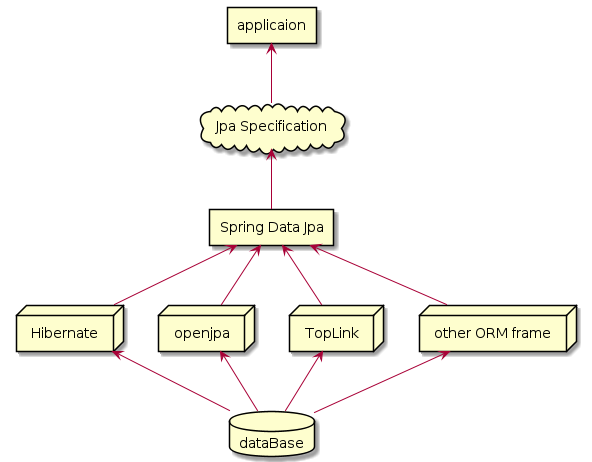
\includegraphics[scale = 0.6]{out/uml/部署图/Jpa和Hibernate/Jpa和Hibernate.png}
              \caption{\song\wuhao Jpa和Hibernate}
              \label{JpaAndHibernate}
          \end{figure}
          Hibernate与MyBatis的对比在一定程度上和Spring Security和Shiro的对比很相似,刚上手Hibernate的感觉,会觉得非常的好用,几乎不用配置就可以使用了,但是随着功能的复杂,需要深入了解复杂的框架本身,对于数据库模型设计的要求也更高,所以Hibernate的学习成本相较于MyBatis更高一些,这是它的缺点,但同时Hibernate的功能更加强大,这是它的优势。\\
          Hibernate特点:
          \begin{enumerate}
              \item 支持自己的“原生”API,同时是JAP的实现,这样,它可以轻松地在支持JPA的任何环境中使用,包括Java SE应用程序,Java EE应用程序服务器,Enterprise OSGi容器等。
              \item 允许按照自然的面向对象的方式进行持久化开发。Hibernate不需要持久化的接口或基类,并且允许任何类或数据持久化。
              \item Hibernate具有较高的性能,它支持延迟初始化,大量的抓取策略和带有自动版本控制和时间戳的乐观锁。无论是开发人员生产方面还是在运行时性能方面,它始终拥有优于直接使用JDBC代码的性能。
              \item Hibernate被设计为在应用服务器集群中工作,并提供高度可伸缩的体系结构。它在任何环境中都可以很好地扩展:使用它来驱动服务于数百个用户地内部网,或者用于服务于数十万用户的关键任务应用程序。
              \item Hibernate拥有卓越的稳定性和质量。
          \end{enumerate}
          总的来说,Hibernate是一个很强大的ORM工具,但是如果想要使用好它,是需要较多的经验的。
\end{enumerate}

\section{Vue.js介绍}

Vue.js特点:
\begin{enumerate}
    \item 轻量级框架\\该框架可以快速下载和安装库。
    \item 虚拟 DOM 渲染及其性能\\
          相关概念:
          \begin{enumerate}
              \item DOM(The Document Object Model):Web页面的API,允许读取和操作页面的内容,结构和样式。一种对HTML基于对象的表示(HTML文档 $\leftrightarrow$ 对象模型)
              \item node tree:DOM的对象结构。
                    \begin{lstlisting} [language = html]
// html
<!doctype html>
<html lang="en">
 <head>
   <title>My first web page</title>
  </head>
 <body>
    <h1>Hello, world!</h1>
    <p>How are you?</p>
  </body>
</html>
          \end{lstlisting}
                    \begin{lstlisting} [language = xml]
// 对应的 node tree
html
|-head
|   |-title
|       |-My first web page
|-body
    |-h1
    |   |-hello,world!
    |-p
        |-How are you?
\end{lstlisting}
              \item Render Tree:(DOM:element的表示 + CSSOM:element样式的表示)
          \end{enumerate}
          虚拟DOM:如果对象更改了它的状态,浏览器需要更新信息并且重新渲染到屏幕上,这个过程需要更新所有的DOM,开销是很大的。而Vue.js利用虚拟DOM解决了这个问题,可以将虚拟DOM理解为DOM的一个拷贝并且它可以找到需要更新的element而不是直接更新所有的element,这大大的提高了应用程序的性能。
    \item 响应式的双向数据绑定(图\ref{tow-way-date-binding})\\
          \begin{figure}[h]
              \centering
              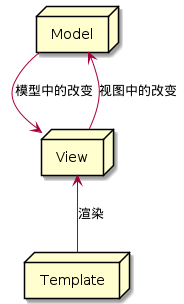
\includegraphics[scale = 0.6]{out/uml/部署图/Two-way data binding/Two-way data binding.png}
              \caption{\song\wuhao 双向数据绑定}
              \label{tow-way-date-binding}
          \end{figure}
    \item CBA\\ Vue是基于组件的体系结构(Component Based Architecture(CBA)),这种体系结构的好处主要有:
          \begin{enumerate}
              \item 代码的可读性:每个组件可以保存在同一个单独的文件,包括结构,样式和逻辑,可以通过代码看出这个组件的功能。
              \item 组件复用:封装好的组件可以再多个地方使用。
              \item 便于单元测试:每个组件刚好可以作为单元测试的一个单元。
          \end{enumerate}
\end{enumerate}

Vue3变化:
\begin{enumerate}
    \item 创建app
          \begin{lstlisting} [language = Java]
// Vue2
import Vue from 'vue'
import App from './App.vue'

Vue.config.productionTip = false

new Vue({
  render: h => h(App),
}).$mount('#app')
    \end{lstlisting}
          \begin{lstlisting} [language = Java]
// Vue3
import { createApp } from 'vue'
import App from './App.vue'
import './index.css'

createApp(App).mount('#app')
    \end{lstlisting}
          改变化解决了Vue2全局配置在单元测试中产生的问题(测试用户会因全局配置而互相影响)
    \item 多Root
\begin{lstlisting} [language = HTML]
<template>
  <div> // 在Vue3中可以去掉
    <h1>{{ msg }}</h1>
    <button @click="count++">count is: {{ count }}</button>
    <p>Edit 
        <code>components/HelloWorld.vue</code> 
      to test hot module replacement.</p>
  </div> // 在Vue3中可以去掉
</template>
\end{lstlisting}
    \item 组合式API。这应该是Vue3最大的变化,该变化主要是为了解决Vue2大组件难以阅读和维护的问题以及管理和维护组件之间的逻辑的问题。主要变化有:
    \begin{enumerate}
        \item Setup
            \begin{lstlisting} [language = HTML]
<template>
  <!-- your template code -->
</template>
<script>
export default {
  setup() {
    // more code to write
  }
};
</script>
            \end{lstlisting}
        \item Reactive References\\
        \lstinline[language = Java]| ref |即"Reactive References",它包装了原始数据并且允许我们跟踪变化。(在Vue2中是使用\lstinline[language = Java]| data() |包装原始内部对象。
        \item Methods/Computed/Watch\\
        Vue2中有一个单独的methods/Computed/Watch部分用来编写方法,在vue3中则在setup()中编写。
        \item Props\\
        在Vue3中不需要this就可以访问props
        \item 移除了Vue filter\\
        在Vue2中filter主要用于普通文本的格式化,而在Vue3中被移除了。移除的主要原因是它的性能和普通的函数没有区别,而写成普通的函数则会有更大的复用空间。
        \item 多个v-model\\
        一个组件可以处理多个v-model,这样在多值处理地情况下,Vue3能更简单地通过多个event将值从子组件传递到父组件。
        \item 模块化
        可以将setup()中的内容分离到另一个composition function中并保存在一个js文件中以便重用。
        \item 声明周期钩子
            \begin{enumerate}
                \item (Vue2)beforeCreate()
                \item (vue2)无$\Rightarrow$(Vue3)setup()
                \item (Vue2)created()
                \item (Vue2)beforeMount()
                \item (Vue2)mounted()
                \item (Vue2)beforeUpdate()
                \item (Vue2)updated()
                \item (Vue2)beforeDestroy()$\Rightarrow$(Vue3)beforeUnmount()
                \item (Vue2)destroyed()$\Rightarrow$(Vue3)unmouted()
                \item (Vue3)onRenderTracked()
                \item (Vue3)onRenderTriggered()
            \end{enumerate}
            并且beforeCreate()和create()不在需要,它们的工作放在setup()中完成。
    \end{enumerate}
\end{enumerate}
